%%%%%%%%%%%%%%%%%%%%%%%%%%%%%%%%%%%%%%%%%%%%%%%%%%%%%%%%%%%%%%%%%%%%%%%%%%%%%%%%
%% LaTeX Vorlage: ergebnisblatt_vorlage.tex                                   %%
%% Dies ist eine Vorlage fuer die Ergebissblaetter zu den Praktikumsaufagben  %%
%% der Vorlesung 'Einfuehrung in das Wissenschaftliche Rechnen'               %%
%%                                                                            %%
%% Version 2020-04-19, F. Castelli (IANM2, KIT)                               %%
%%%%%%%%%%%%%%%%%%%%%%%%%%%%%%%%%%%%%%%%%%%%%%%%%%%%%%%%%%%%%%%%%%%%%%%%%%%%%%%%
\documentclass[11pt,a4paper]{article}


%% Pakete
\usepackage[ngerman]{babel}
\usepackage[T1]{fontenc}
\usepackage[utf8]{inputenc}   % Unix
% \usepackage[latin1]{inputenc} % Windows
\usepackage[pdftex]{graphicx}
\usepackage{epstopdf}
\usepackage{amsmath,amssymb}
\usepackage{caption}



%% Seitenlayout
\usepackage[DIV=12]{typearea}
\setlength{\parindent}{0em}


%% Font Helvetica
\renewcommand{\rmdefault}{phv}


%% Titelinformationen
\title{Einf\"uhrung in das Wissenschaftliche Rechnen\\
  Praktikumsblatt 10\\
  Aufgabe 22 (Singuläre Lösung)}
\author{Lena Hilpp Matr.Nr.: 1941997 \\ Jan Frithjof Fleischhammer Matr.Nr.: 2115491}
\date{09.07.2020}



%%%%%%%%%%%%%%%%%%%%%%%%%%%%%%%%%%%%%%%%%%%%%%%%%%%%%%%%%%%%%%%%%%%%%%%%%%%%%%%%
\begin{document}
  
  %% Titel
  \maketitle
  
  %%%%%%%%%%%%%%%%%%%%%%%%%%%%%%%%%%%%%%%%%%%%%%%%%%%%%%%%%%%%%%%%%%%%%%%%%%%%%%
  \section*{Problemstellung}
  %%%%%%%%%%%%%%%%%%%%%%%%%%%%%%%%%%%%%%%%%%%%%%%%%%%%%%%%%%%%%%%%%%%%%%%%%%%%%%
 
 
 In dieser Aufgabe betrachtet man das Poisson-Problem
 \begin{equation}
\begin{cases}
 -\Delta u = f  & \text{ in } \Omega \\
\qquad u = u^D  & \text{ auf } \partial\Omega, 
 \end{cases}
 \label{1}
 \end{equation}
 
wobei $\Omega$ ein Gebiet mit einspringender Ecke ist. Die rechte Seite $f$ und die inhomogene Dirichlet-Randbedingungen von (\ref{1}) werden so gewählt, dass die exakte Lösung des Problems, in Polarkoordinaten, durch 
\begin{align*}
u(r,\phi)=r^{2/3}\cos \left(\frac{2}{3} \phi\right)
\end{align*}
gegeben ist. Daraus ergibt sich $f=0$.\\
Mit Hilfe der Finiten-Elemente-Methode wird eine numerische Lösung berechnet und die experientelle Konvergenzordnung bestimmt.
  
  %%%%%%%%%%%%%%%%%%%%%%%%%%%%%%%%%%%%%%%%%%%%%%%%%%%%%%%%%%%%%%%%%%%%%%%%%%%%%%
  \section*{Ergebnis}
  %%%%%%%%%%%%%%%%%%%%%%%%%%%%%%%%%%%%%%%%%%%%%%%%%%%%%%%%%%%%%%%%%%%%%%%%%%%%%%
   In \textit{Abbildung \ref{Abb1}} sieht man beispielhaft zwei unterschiedlich feine Gitter auf denen die Lösung berechnet wurde. Als Triangulierung wurde hier \textit{Criss-Cross} verwendet.  
  
  \begin{center}
  \begin{tabular}{cc}
  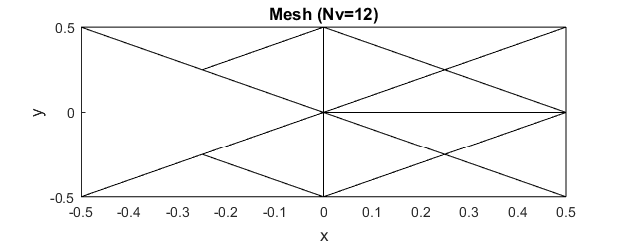
\includegraphics[width=0.5\textwidth]{Gitter2}&
  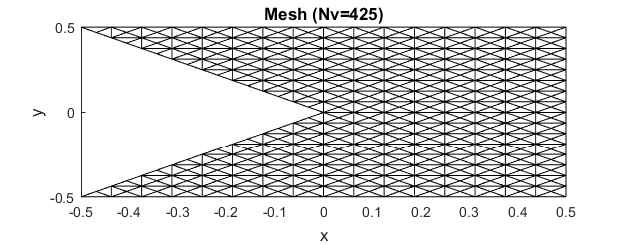
\includegraphics[width=0.5\textwidth]{Gitter1}\\ 
  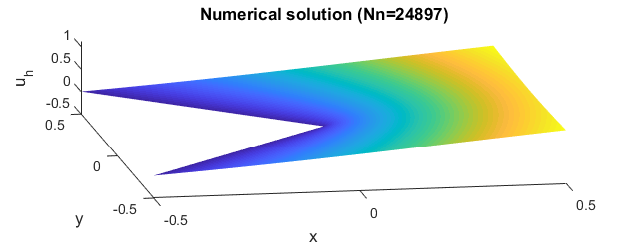
\includegraphics[width=0.5\textwidth]{Loesung}
   \end{tabular}
  \captionof{figure}{unterschiedlich feine Gitter und numerische Lösung $u_h$}
  \label{Abb1}
  \end{center}

  Für $N=[2;4;8;16]$ (Anzahl der Zellen pro Dimension) ist in \textit{Abbildung \ref{Abb2}}, für verschiedene Polynomgrade, die experimentelle Konvergenzordnung graphisch aufgetragen.
   \begin{center}
  \begin{tabular}{cc}
  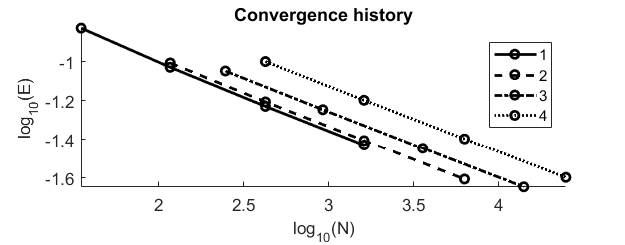
\includegraphics[width=0.8\textwidth]{konv}
   \end{tabular}
  \captionof{figure}{Konvergenz für pd=[2,4,6,8]}
  \label{Abb2}
  \end{center}
  
  Der geschätzte Fehler für Polynomgrad $2$ liegt bei $ E = 4.80\times 10^{-1} * h^{ 0.69}$ und bei Polynomgrad $8$ bei $E = 7.58\times 10^{-1} * h^{ 0.67}$. Erwartet haben wir allerdings etwas anderes. In der Theorie sollte der Polynomgrad in etwa der Ordnung entsprechen. Diese beobachteten Konvergenzordnungen stehen trotzdem nicht im Widerspruch zur theoretischen Fehlerschranke der Finite-Elemente-Methode, da wir hier ein Gebiet mit einspringender Ecke betrachten und deshalb die exakte Lösung auf dem Gebiet nicht stetig differenzierbar ist. \\ 

 Anstatt das Gitter in jedem Schritt global zu verfeinern wurde nun eine adaptive Gitterverfeinerung verwendet. Dadurch erhält man die Konvergenz Ordnung die in \textit{Abbildung \ref{Abb3}} abgebildet ist. Der geschätzte Fehler berägt $E=2.08*h^{0.662}$ für $pd=1$. Es gilt ca. $ERR \sim N^{eoc/2}$.

\begin{center}
  \begin{tabular}{cc}
  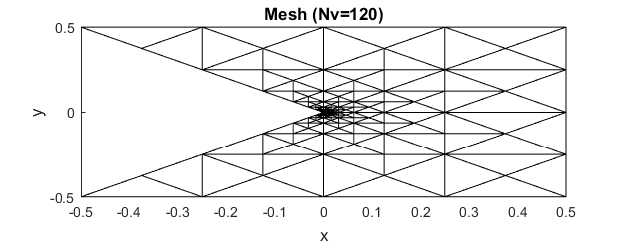
\includegraphics[width=0.5\textwidth]{Gitter3}&
  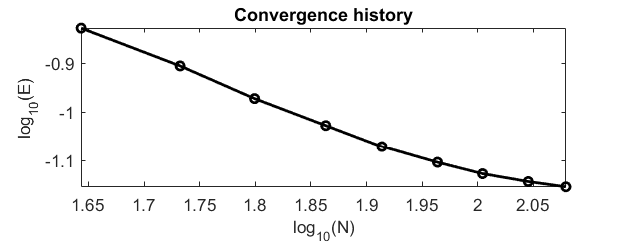
\includegraphics[width=0.5\textwidth]{EOC}
   \end{tabular}
  \captionof{figure}{adaptive Gitterverfeinerung und Konvergenz History}
  \label{Abb3}
  \end{center}
  



\end{document}